\documentclass[border=8pt]{standalone}
\usepackage[T1]{fontenc}\usepackage{helvet}\renewcommand{\familydefault}{\sfdefault}
\usepackage{tikz}\usetikzlibrary{arrows.meta, positioning, calc, backgrounds}
\definecolor{ink}{HTML}{1a1916}
\definecolor{inktwo}{HTML}{3a3a35}
\definecolor{inkthree}{HTML}{6a6862}
\definecolor{rule}{HTML}{b8b09a}
\definecolor{amber}{HTML}{a8730a}
\definecolor{red}{HTML}{c8261a}
\definecolor{paper}{HTML}{f0eee5}
\definecolor{slab}{HTML}{d8d4c6}
\tikzset{
  >={Stealth[length=2.2mm]},
  wire/.style={line width=0.8pt, ink},
  modwire/.style={line width=0.6pt, dashed, ink},
  tastewire/.style={line width=0.6pt, dashed, amber},
  gatewire/.style={line width=0.6pt, dotted, ink},
  block/.style={rectangle, draw=ink, line width=0.9pt, fill=slab, minimum width=3.0cm, minimum height=1.9cm, inner sep=0pt},
  perf/.style={rectangle, draw=ink, line width=0.7pt, minimum width=3.0cm, minimum height=0.7cm, inner sep=2pt, font=\footnotesize, text=ink},
  title/.style={font=\scriptsize\bfseries, text=ink, anchor=north, inner sep=2pt},
  jack/.style={circle, draw=ink, fill=paper, line width=0.5pt, minimum size=3.2pt, inner sep=0pt},
  plabel/.style={font=\tiny, text=inktwo, anchor=west, inner sep=1pt},
  olabel/.style={font=\tiny, text=inktwo, anchor=east, inner sep=1pt},
  settings/.style={font=\scriptsize, text=ink, align=left, anchor=north west, inner sep=1pt, text width=2.9cm},
}
\begin{document}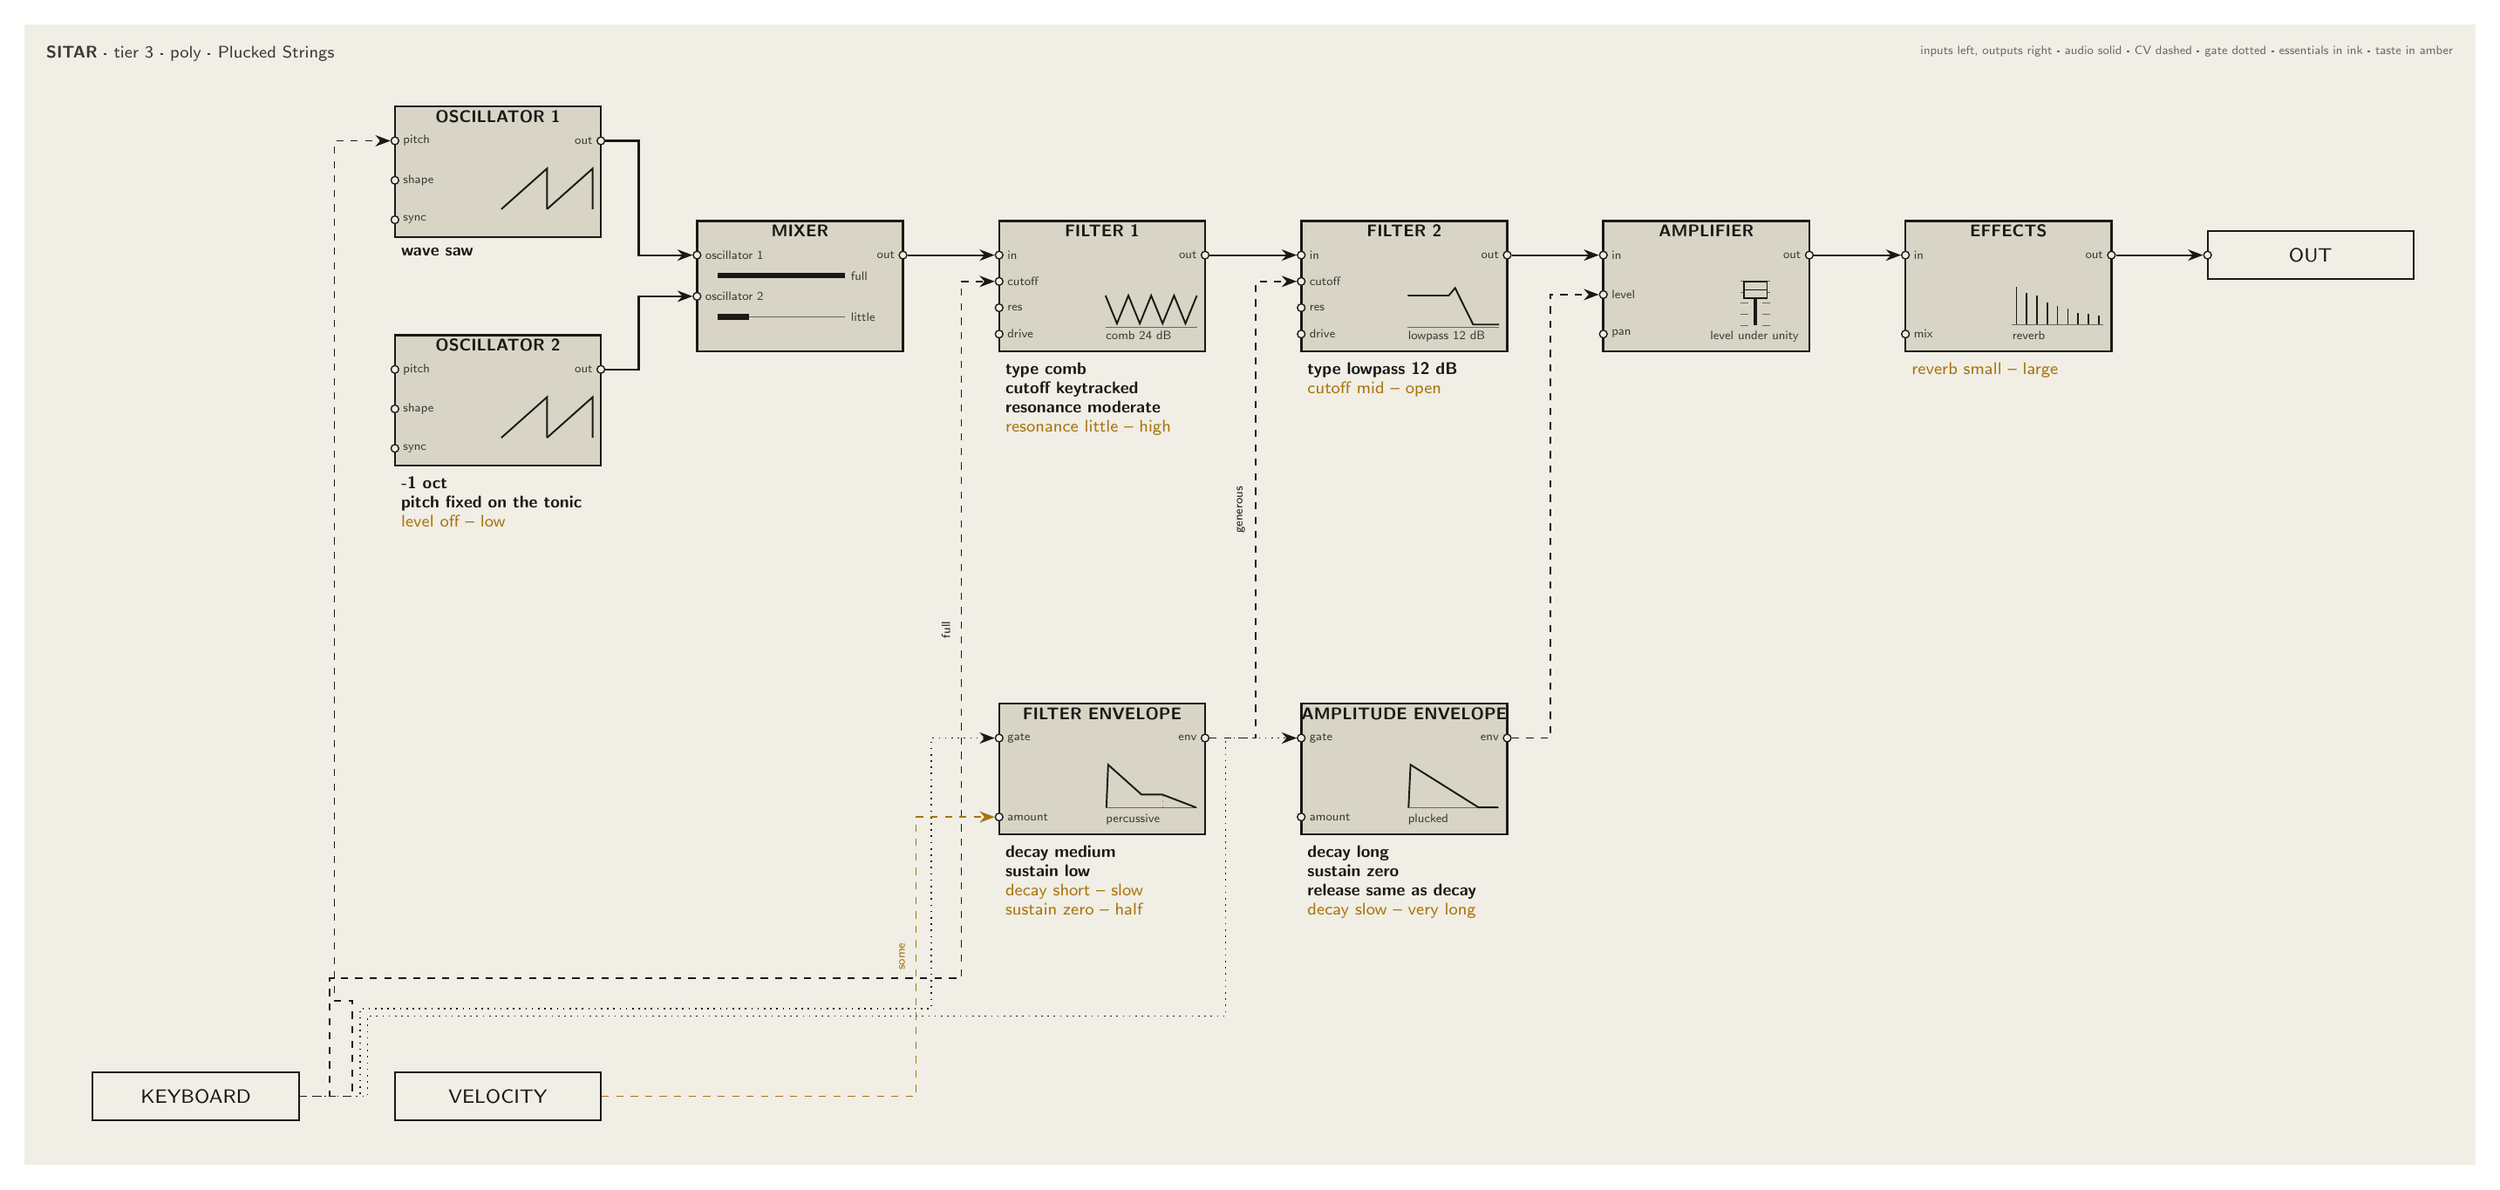
\begin{tikzpicture}
\begin{scope}[on background layer]\fill[paper] (-2.5,-12.805) rectangle (33.2,3.8150000000000004);\end{scope}
\node[block, minimum height=1.9cm] (osc1) at (4.4,1.665) {};
\node[title] at (osc1.north) {OSCILLATOR 1};
\node[jack] (osc1-pitch) at (2.9000000000000004,2.115) {};
\node[plabel] at (2.9800000000000004,2.115) {pitch};
\node[jack] (osc1-shape) at (2.9000000000000004,1.5400000000000003) {};
\node[plabel] at (2.9800000000000004,1.5400000000000003) {shape};
\node[jack] (osc1-sync) at (2.9000000000000004,0.9650000000000003) {};
\node[plabel] at (2.9800000000000004,0.9650000000000003) {sync};
\node[jack] (osc1-out) at (5.9,2.115) {};
\node[olabel] at (5.82,2.115) {out};
\begin{scope}
\draw[ink, line width=0.7pt] (4.450,1.119) -- (5.115,1.711) -- (5.115,1.119);
\draw[ink, line width=0.7pt] (5.115,1.119) -- (5.780,1.711) -- (5.780,1.119);
\end{scope}
\node[settings] at (2.95,0.5950000000000001) {\textbf{wave saw}};
\node[block, minimum height=1.9cm] (osc2) at (4.4,-1.665) {};
\node[title] at (osc2.north) {OSCILLATOR 2};
\node[jack] (osc2-pitch) at (2.9000000000000004,-1.215) {};
\node[plabel] at (2.9800000000000004,-1.215) {pitch};
\node[jack] (osc2-shape) at (2.9000000000000004,-1.79) {};
\node[plabel] at (2.9800000000000004,-1.79) {shape};
\node[jack] (osc2-sync) at (2.9000000000000004,-2.365) {};
\node[plabel] at (2.9800000000000004,-2.365) {sync};
\node[jack] (osc2-out) at (5.9,-1.215) {};
\node[olabel] at (5.82,-1.215) {out};
\begin{scope}
\draw[ink, line width=0.7pt] (4.450,-2.211) -- (5.115,-1.619) -- (5.115,-2.211);
\draw[ink, line width=0.7pt] (5.115,-2.211) -- (5.780,-1.619) -- (5.780,-2.211);
\end{scope}
\node[settings] at (2.95,-2.7350000000000003) {\textbf{-1 oct} \\ \textbf{pitch fixed on the tonic} \\ \textcolor{amber}{level off -- low}};
\node[block, minimum height=1.9cm] (mix) at (8.8,0.0) {};
\node[title] at (mix.north) {MIXER};
\node[jack] (mix-osc1) at (7.300000000000001,0.44999999999999996) {};
\node[plabel] at (7.380000000000001,0.44999999999999996) {oscillator 1};
\draw[inkthree, line width=0.3pt] (7.600,0.150) -- (9.450,0.150);
\draw[ink, line width=2.2pt] (7.600,0.150) -- (9.450,0.150);
\node[font=\tiny, text=inktwo, anchor=west, inner sep=1pt] at (9.500,0.150) {full};
\node[jack] (mix-osc2) at (7.300000000000001,-0.15000000000000002) {};
\node[plabel] at (7.380000000000001,-0.15000000000000002) {oscillator 2};
\draw[inkthree, line width=0.3pt] (7.600,-0.450) -- (9.450,-0.450);
\draw[ink, line width=2.2pt] (7.600,-0.450) -- (8.062,-0.450);
\node[font=\tiny, text=inktwo, anchor=west, inner sep=1pt] at (9.500,-0.450) {little};
\node[jack] (mix-out) at (10.3,0.44999999999999996) {};
\node[olabel] at (10.22,0.44999999999999996) {out};
\node[block, minimum height=1.9cm] (filter1) at (13.200000000000001,0.0) {};
\node[title] at (filter1.north) {FILTER 1};
\node[jack] (filter1-in) at (11.700000000000001,0.44999999999999996) {};
\node[plabel] at (11.780000000000001,0.44999999999999996) {in};
\node[jack] (filter1-cutoff) at (11.700000000000001,0.06666666666666665) {};
\node[plabel] at (11.780000000000001,0.06666666666666665) {cutoff};
\node[jack] (filter1-res) at (11.700000000000001,-0.31666666666666665) {};
\node[plabel] at (11.780000000000001,-0.31666666666666665) {res};
\node[jack] (filter1-drive) at (11.700000000000001,-0.7) {};
\node[plabel] at (11.780000000000001,-0.7) {drive};
\node[jack] (filter1-out) at (14.700000000000001,0.44999999999999996) {};
\node[olabel] at (14.620000000000001,0.44999999999999996) {out};
\begin{scope}
\draw[inkthree, line width=0.3pt] (13.250,-0.605) -- (14.580,-0.605);
\draw[ink, line width=0.7pt] (13.250,-0.139) -- (13.416,-0.546) -- (13.583,-0.139) -- (13.749,-0.546) -- (13.915,-0.139) -- (14.081,-0.546) -- (14.248,-0.139) -- (14.414,-0.546) -- (14.580,-0.139);
\node[font=\tiny, text=inktwo, anchor=north west, inner sep=0pt] at (13.250,-0.650) {comb 24 dB};
\end{scope}
\node[settings] at (11.750000000000002,-1.0699999999999998) {\textbf{type comb} \\ \textbf{cutoff keytracked} \\ \textbf{resonance moderate} \\ \textcolor{amber}{resonance little -- high}};
\node[block, minimum height=1.9cm] (filter2) at (17.6,0.0) {};
\node[title] at (filter2.north) {FILTER 2};
\node[jack] (filter2-in) at (16.1,0.44999999999999996) {};
\node[plabel] at (16.18,0.44999999999999996) {in};
\node[jack] (filter2-cutoff) at (16.1,0.06666666666666665) {};
\node[plabel] at (16.18,0.06666666666666665) {cutoff};
\node[jack] (filter2-res) at (16.1,-0.31666666666666665) {};
\node[plabel] at (16.18,-0.31666666666666665) {res};
\node[jack] (filter2-drive) at (16.1,-0.7) {};
\node[plabel] at (16.18,-0.7) {drive};
\node[jack] (filter2-out) at (19.1,0.44999999999999996) {};
\node[olabel] at (19.020000000000003,0.44999999999999996) {out};
\begin{scope}
\draw[inkthree, line width=0.3pt] (17.650,-0.605) -- (18.980,-0.605);
\draw[ink, line width=0.7pt] (17.650,-0.139) -- (18.248,-0.139) -- (18.342,-0.028) -- (18.395,-0.139) -- (18.604,-0.561) -- (18.980,-0.561);
\node[font=\tiny, text=inktwo, anchor=north west, inner sep=0pt] at (17.650,-0.650) {lowpass 12 dB};
\end{scope}
\node[settings] at (16.150000000000002,-1.0699999999999998) {\textbf{type lowpass 12 dB} \\ \textcolor{amber}{cutoff mid -- open}};
\node[block, minimum height=1.9cm] (amp) at (22.0,0.0) {};
\node[title] at (amp.north) {AMPLIFIER};
\node[jack] (amp-in) at (20.5,0.44999999999999996) {};
\node[plabel] at (20.58,0.44999999999999996) {in};
\node[jack] (amp-level) at (20.5,-0.125) {};
\node[plabel] at (20.58,-0.125) {level};
\node[jack] (amp-pan) at (20.5,-0.7) {};
\node[plabel] at (20.58,-0.7) {pan};
\node[jack] (amp-out) at (23.5,0.44999999999999996) {};
\node[olabel] at (23.42,0.44999999999999996) {out};
\begin{scope}
\draw[ink, line width=1.2pt] (22.715,-0.570) -- (22.715,0.070);
\draw[inkthree, line width=0.3pt] (22.495,-0.570) -- (22.615,-0.570) (22.815,-0.570) -- (22.935,-0.570);
\draw[inkthree, line width=0.3pt] (22.495,-0.410) -- (22.615,-0.410) (22.815,-0.410) -- (22.935,-0.410);
\draw[inkthree, line width=0.3pt] (22.495,-0.250) -- (22.615,-0.250) (22.815,-0.250) -- (22.935,-0.250);
\draw[inkthree, line width=0.3pt] (22.495,-0.090) -- (22.615,-0.090) (22.815,-0.090) -- (22.935,-0.090);
\draw[inkthree, line width=0.3pt] (22.495,0.070) -- (22.615,0.070) (22.815,0.070) -- (22.935,0.070);
\fill[slab, draw=ink, line width=0.6pt] (22.545,-0.178) rectangle (22.885,0.062);
\draw[ink, line width=0.5pt] (22.545,-0.058) -- (22.885,-0.058);
\node[font=\tiny, text=inktwo, anchor=north west, inner sep=0pt] at (22.050,-0.650) {level under unity};
\end{scope}
\node[block, minimum height=1.9cm] (fx) at (26.400000000000002,0.0) {};
\node[title] at (fx.north) {EFFECTS};
\node[jack] (fx-in) at (24.900000000000002,0.44999999999999996) {};
\node[plabel] at (24.98,0.44999999999999996) {in};
\node[jack] (fx-mix) at (24.900000000000002,-0.7) {};
\node[plabel] at (24.98,-0.7) {mix};
\node[jack] (fx-out) at (27.900000000000002,0.44999999999999996) {};
\node[olabel] at (27.820000000000004,0.44999999999999996) {out};
\begin{scope}
\draw[inkthree, line width=0.3pt] (26.450,-0.561) -- (27.780,-0.561);
\draw[ink, line width=0.6pt] (26.517,-0.561) -- (26.517,-0.018);
\draw[ink, line width=0.6pt] (26.666,-0.561) -- (26.666,-0.095);
\draw[ink, line width=0.6pt] (26.816,-0.561) -- (26.816,-0.133);
\draw[ink, line width=0.6pt] (26.965,-0.561) -- (26.965,-0.246);
\draw[ink, line width=0.6pt] (27.115,-0.561) -- (27.115,-0.296);
\draw[ink, line width=0.6pt] (27.265,-0.561) -- (27.265,-0.335);
\draw[ink, line width=0.6pt] (27.414,-0.561) -- (27.414,-0.394);
\draw[ink, line width=0.6pt] (27.564,-0.561) -- (27.564,-0.408);
\draw[ink, line width=0.6pt] (27.713,-0.561) -- (27.713,-0.429);
\node[font=\tiny, text=inktwo, anchor=north west, inner sep=0pt] at (26.450,-0.650) {reverb};
\end{scope}
\node[settings] at (24.950000000000003,-1.0699999999999998) {\textcolor{amber}{reverb small -- large}};
\node[block, minimum height=1.9cm] (fenv) at (13.200000000000001,-7.035000000000001) {};
\node[title] at (fenv.north) {FILTER ENVELOPE};
\node[jack] (fenv-gate) at (11.700000000000001,-6.585000000000001) {};
\node[plabel] at (11.780000000000001,-6.585000000000001) {gate};
\node[jack] (fenv-amount) at (11.700000000000001,-7.735000000000001) {};
\node[plabel] at (11.780000000000001,-7.735000000000001) {amount};
\node[jack] (fenv-out) at (14.700000000000001,-6.585000000000001) {};
\node[olabel] at (14.620000000000001,-6.585000000000001) {env};
\begin{scope}
\draw[inkthree, line width=0.3pt] (13.250,-7.596) -- (14.580,-7.596);
\draw[ink, line width=0.7pt] (13.263,-7.596) -- (13.288,-6.974) -- (13.775,-7.409) -- (14.079,-7.409) -- (14.567,-7.596);
\draw[inkthree, line width=0.3pt, dotted] (14.079,-7.596) -- (14.079,-7.409);
\node[font=\tiny, text=inktwo, anchor=north west, inner sep=0pt] at (13.250,-7.685) {percussive};
\end{scope}
\node[settings] at (11.750000000000002,-8.105) {\textbf{decay medium} \\ \textbf{sustain low} \\ \textcolor{amber}{decay short -- slow} \\ \textcolor{amber}{sustain zero -- half}};
\node[block, minimum height=1.9cm] (aenv) at (17.6,-7.035000000000001) {};
\node[title] at (aenv.north) {AMPLITUDE ENVELOPE};
\node[jack] (aenv-gate) at (16.1,-6.585000000000001) {};
\node[plabel] at (16.18,-6.585000000000001) {gate};
\node[jack] (aenv-amount) at (16.1,-7.735000000000001) {};
\node[plabel] at (16.18,-7.735000000000001) {amount};
\node[jack] (aenv-out) at (19.1,-6.585000000000001) {};
\node[olabel] at (19.020000000000003,-6.585000000000001) {env};
\begin{scope}
\draw[inkthree, line width=0.3pt] (17.650,-7.596) -- (18.980,-7.596);
\draw[ink, line width=0.7pt] (17.663,-7.596) -- (17.692,-6.974) -- (18.683,-7.596) -- (18.683,-7.596) -- (18.967,-7.596);
\node[font=\tiny, text=inktwo, anchor=north west, inner sep=0pt] at (17.650,-7.685) {plucked};
\end{scope}
\node[settings] at (16.150000000000002,-8.105) {\textbf{decay long} \\ \textbf{sustain zero} \\ \textbf{release same as decay} \\ \textcolor{amber}{decay slow -- very long}};
\node[perf] (key) at (0.0,-11.805) {KEYBOARD};
\node[perf] (vel) at (4.4,-11.805) {VELOCITY};
\node[perf, fill=paper] (out) at (30.800000000000004,0.44999999999999996) {OUT}; \node[jack] (out-in) at (29.300000000000004,0.44999999999999996) {};
\draw[wire,->] (osc1-out) -- (6.45,2.115) |- (mix-osc1);
\draw[wire,->] (osc2-out) -- (6.45,-1.215) |- (mix-osc2);
\draw[wire,->] (mix-out) -- (filter1-in);
\draw[wire,->] (filter1-out) -- (filter2-in);
\draw[wire,->] (filter2-out) -- (amp-in);
\draw[wire,->] (amp-out) -- (fx-in);
\draw[wire,->] (fx-out) -- (out-in);
\draw[modwire,->] (key.east) -- (1.95,-11.805) -- (1.95,-10.085) -- (11.15,-10.085) -- (11.15,0.06666666666666665) -- (filter1-cutoff);
\node[font=\tiny, text=ink, anchor=south, inner sep=1pt, rotate=90] at (11.030000000000001,-5.009166666666667) {full};
\draw[modwire,->] (fenv-out) -- (15.440000000000001,-6.585000000000001) -- (15.440000000000001,0.06666666666666665) -- (filter2-cutoff);
\node[font=\tiny, text=ink, anchor=south, inner sep=1pt, rotate=90] at (15.320000000000002,-3.259166666666667) {generous};
\draw[modwire,->] (aenv-out) -- (19.73,-6.585000000000001) -- (19.73,-0.125) -- (amp-level);
\draw[modwire,->] (key.east) -- (2.28,-11.805) -- (2.28,-10.415000000000001) -- (2.0200000000000005,-10.415000000000001) -- (2.0200000000000005,2.115) -- (osc1-pitch);
\draw[gatewire,->] (key.east) -- (2.39,-11.805) -- (2.39,-10.525) -- (10.71,-10.525) -- (10.71,-6.585000000000001) -- (fenv-gate);
\draw[gatewire,->] (key.east) -- (2.5,-11.805) -- (2.5,-10.635000000000002) -- (15.0,-10.635000000000002) -- (15.0,-6.585000000000001) -- (aenv-gate);
\draw[tastewire,->] (vel.east) -- (10.49,-11.805) -- (10.49,-7.735000000000001) -- (fenv-amount);
\node[font=\tiny, text=amber, anchor=south, inner sep=1pt, rotate=90] at (10.370000000000001,-9.77) {some};
\node[anchor=north west, font=\scriptsize, text=inktwo] at (-2.3,3.615) {\textbf{SITAR} · tier 3 · poly · Plucked Strings};
\node[anchor=north east, font=\tiny, text=inkthree] at (33.0,3.615) {inputs left, outputs right · audio solid · CV dashed · gate dotted · essentials in ink · taste in amber};
\end{tikzpicture}\end{document}
